%%%%%%%%%%%%%%%%%%%%%%%%%%%%%
% Standard header for working papers
%
% WPHeader.tex
%
%%%%%%%%%%%%%%%%%%%%%%%%%%%%%


%%%%%%%%%%%%%%%%%%%%%%%%%%
%% TEMPLATES
%%%%%%%%%%%%%%%%%%%%%%%%%%


% Simple Tabular

%\begin{tabular}{ |c|c|c| } 
% \hline
% cell1 & cell2 & cell3 \\ 
% cell4 & cell5 & cell6 \\ 
% cell7 & cell8 & cell9 \\ 
% \hline
%\end{tabular}







\documentclass[11pt]{article}

%%%%%%%%%%%%%%%%%%%%
%% Include general header where common packages are defined
%%%%%%%%%%%%%%%%%%%%



%%%%%%%%%%%%%%%%%%%%%%%%%%
%% Packages
%%%%%%%%%%%%%%%%%%%%%%%%%%


% general packages without options
\usepackage{amsmath,amssymb,bbm}

% graphics
\usepackage{graphicx}

\usepackage{pdfpages}

% text formatting
\usepackage[document]{ragged2e}
\usepackage{pagecolor,color,setspace}




\usepackage[utf8]{inputenc}
\usepackage[T1]{fontenc}
%\usepackage[francais]{babel}



% for framed figures or texts
\usepackage{mdframed}



%%%%%%%%%%%%%%%%%%%%
%% Idem general commands
%%%%%%%%%%%%%%%%%%%%
%% Commands

\newcommand{\noun}[1]{\textsc{#1}}


%% Math

% Operators
\DeclareMathOperator{\Cov}{Cov}
\DeclareMathOperator{\Var}{Var}
\DeclareMathOperator{\E}{\mathbb{E}}
\DeclareMathOperator{\Proba}{\mathbb{P}}

\newcommand{\Covb}[2]{\ensuremath{\Cov\!\left[#1,#2\right]}}
\newcommand{\Eb}[1]{\ensuremath{\E\!\left[#1\right]}}
\newcommand{\Pb}[1]{\ensuremath{\Proba\!\left[#1\right]}}
\newcommand{\Varb}[1]{\ensuremath{\Var\!\left[#1\right]}}

% norm
\newcommand{\norm}[1]{\| #1 \|}


%% graphics

% renew graphics command for relative path providment only ?
%\renewcommand{\includegraphics[]{}}



% geometry
\usepackage[margin=2cm]{geometry}

\usepackage{float}

% layout : use fancyhdr package
\usepackage{fancyhdr}
\pagestyle{fancy}

\makeatletter

\renewcommand{\headrulewidth}{0.4pt}
\renewcommand{\footrulewidth}{0.4pt}
\fancyhead[RO,RE]{04/2017}
\fancyhead[LO,LE]{Réseaux et Territoires}
\fancyfoot[RO,RE] {\thepage}
\fancyfoot[LO,LE] {L2 Analyse Spatiale - 2016-2017}
\fancyfoot[CO,CE] {}


\fancypagestyle{firststyle}
{
   \fancyhf{}
   \fancyhead[RO,RE]{TD6 - 04/2017}
   \fancyhead[LO,LE]{L2 Analyse Spatiale - 2016-2017}
}


\renewcommand{\abstractname}{Résumé}

\renewcommand{\figurename}{\textbf{Document}}

\newcommand{\question}[1]{$\rightarrow$ \textit{#1}}


\makeatother


%%%%%%%%%%%%%%%%%%%%%
%% Begin doc
%%%%%%%%%%%%%%%%%%%%%

\begin{document}









\title{\textbf{TD6 : Réseaux et Territoires}}

\date{}


\maketitle

\justify

\thispagestyle{firststyle}

%\vspace{-1cm}

\justify

\begin{abstract}
\noindent
Ce TD propose une ouverture sur les relations complexes entre réseaux et territoires, pour appréhender la multiplicité et la complémentarité des approches possibles, et comprendre l'importance des notions vues en cours dans la plupart de celles-ci.
%$\rightarrow$ Aborder la notion de réseau en géographie.
%\smallskip\vspace{-0.1cm}\\
%$\rightarrow$ Acquérir des notions de base d'analyse des réseaux.
%\medskip\\$\rightarrow$ Aborder les relations complexes entre réseaux et territoires.
\end{abstract}


\bigskip
\bigskip


\section{Introduction : des relations complexes}



\hspace{16pt}\question{A partir du document~\ref{doc:offner-pumain}, proposez des processus capturant l'influence des réseaux de transport sur les territoires. Proposez également les impacts possibles d'autres types de réseaux sur les territoires. Reliez si possible ces processus à des notions vues en cours (accessibilité, centralité, \ldots)}

\medskip

\question{A partir de vos connaissances, donnez des processus inverses d'influence des territoires sur la croissance des réseaux de transport.}

\medskip

\question{Etant donné les interactions réciproques à différentes échelles que vous avez identifié, discutez la complexité de l'évolution du système réseaux-territoires.}


\begin{figure}[h!]
\begin{mdframed}
\centering\justify
\textbf{L’impact socio-économique des réseaux de transport}

\medskip

Comment se traduisent les changements successifs de
l'accessibilité sur la dynamique socio—économique des territoires concernés ? C’est essentiellement à l’occasion de la mise
en service des infrastructures que ces effets sont susceptibles
d'être observés. C’est à ce moment-la qu'elles créent, par leur
presence et leur absence, des discriminations bien perceptibles
entre lieux, discriminations qui s'estompent d’ailleurs au fur et
à mesure de leur diffusion spatiale. Ce problème n’a fait l’objet
d’étude que récemment, avec le développement des autoroutes et du TGV, de la part des titulaires de ces réseaux d'une
part, et de chercheurs d’autre part.

\medskip

\textit{Les effets des réseaux}

\medskip

La question des effets des réseaux a été posée tout d'abord
dans une optique d’aménagement du territoire à l’échelon de la
France, puis au niveau européen. Ces effets ont été identifiés
en fonction du terme ou ils apparaissent.

A court et moyen termes (moins de cinq ans), outre les
effets de construction (relance du secteur des travaux publics)
qui ne sont pas spécifiques au domaine des transports, il y a les
effets directs, ou consequences de la mise en service d’une
infrastructure sur ses usagers anciens ou nouveaux. Ces effets
se traduisent soit en termes de report d’un mode sur l’autre,
comme le transfert de l’aérien sur le TGV Sud-Est, soit en
termes de trafic induit. A titre d’exemple, des usagers anciens
sont incités à préférer plusieurs allers et retours journaliers à
un séjour prolongé. Ces effets ont tous un caractère mécanique, car liés aux variations de trafic. Les activités concernées sont celles qui sont liées au transport, telles que l'hôtellerie ou la
restauration, le rabattement sur les gares assure par les autocaristes, les taxis, les loueurs de voiture... A long terme, il s’agit
d'effets indirects, transformations entrainées par la nouvelle
infrastructure sur l'organisation des activités et leur répartition spatiale. Ils sont très divers, pouvant se traduire par de
nouvelles localisations d’activités industrielles ou tertiaires,
un développement du tourisme et de l’immobilier dans les
régions desservies. Ils sont plus lents et plus incertains que
les deux premiers, car ils transitent par les comportements des
agents économiques dont l’inertie est beaucoup plus grande
que celle des pratiques de mobilité. Quant à la question des
liens entre effets directs et effets indirects, elle n’est point encore élucidée.


Ces effets de long terme sont désignés par les promoteurs de ces équipements sous le nom d’effets structurants, c’est-à-
dire suffisants pour impulser des dynamiques nouvelles entrainant un changement structurel. Afin de pouvoir justifier d’un
impact bénéfique des dépenses qui sont décidées, il convient
de faire apparaitre ces équipements comme moteur dc développement économique et social, en dégageant une relation de cause à effet. Cette notion d’effet structurant est cependant
battue en brèche par un certain nombre de chercheurs dans la
mesure où leurs travaux convergent pour en dénoncer l’absence de validation scientifique.


\end{mdframed}

\caption{\textbf{Impact des infrastructures de transport.} Source : Offner, J. M., \& Pumain, D. (1996). Réseaux et territoires-significations croisées.}
\label{doc:offner-pumain}

\end{figure}




%%%%%%%%%%%%%%%%%%
\section{Vers une modélisation intégrée des interactions entre réseaux et territoires}
%%%%%%%%%%%%%%%%%%

On se propose de brosser un aperçu de recherches courantes, visant à construire des modélisations intégrées de la croissance des réseaux et des territoires, dans le cas particulier des réseaux de transport et majoritairement des villes. On essaye de rendre compte de la diversité des points de vue et approches possibles. Une étude bibliométrique préliminaire suggère l'organisation des domaines scientifiques s'intéressant au problème, étape nécessaire pour comprendre les enjeux thématiques des modèles potentiels. A l'échelle microscopique, l'étude de la congestion dans un réseau routier révèle la nature chaotique des interactions. A l'échelle mesoscopique, les correlations entre forme urbaine et indicateurs de réseaux suggèrent une variété de régimes d'interaction, ce qui est confirmé par une étude systématique de régime de causalité sur un modèle simple de morphogenèse urbaine. Enfin, l'échelle macroscopique témoigne d'effets de réseaux pouvant être interprétés comme des effets de structure.


%%%%%%%%%%%%%%%%%%
\subsection{Analyse bibliométrique : quels positionnement disciplinaires ?}

Les interactions entre réseaux de transport et territoires sont des objets pouvant être étudiés du point de vue de nombreuses disciplines, et avec des ontologies variées : géographie urbaine, géographie des réseaux, économie des transports, économie des réseaux, aménagement, planification urbaine, physique, etc. Une étape préliminaire effectuée par \cite{raimbault2015models} consiste à extraire de manière quantifiée la structure de ces disciplines. Un algorithme procède par itérations, partant de mots clés initiaux, récupère les références correspondantes dans un catalogue, extrait des nouveaux mot-clés par analyse textuelle, et répète l'opération jusqu'à obtenir un corpus stabilisé. Un traitement complémentaire s'intéresse au réseau de citations connecté à des références de base.

\medskip

\question{Commentez les résultats de proximité des corpus finaux du document~\ref{fig:algosr} ; quelles sont leur implications pour une quantification de proximités disciplinaires ?}

\medskip

% réseau de citations : communautés ?
\question{Commentez le réseau de citations présenté en document~\ref{fig:citnw}, en mobilisant les notions sur les graphes vues en cours. Dans quelle mesure l'analyse des communautés peut-elle renforcer les conclusions précédentes ?}





%%%%%%%%%%%%%%%
\begin{figure}
\centering
\includegraphics[width=0.48\textwidth]{figures/biblio_structure}
\includegraphics[width=0.48\textwidth]{figures/biblio_results}
\caption{\textbf{Revue systématique algorithmique.} \textbf{(Gauche)} Architecture de l'algorithme d'exploration sémantique de la littérature. Etant donné un ensemble de mots-clés $\mathcal{K}_n$, une requête à un catalogue donne un corpus de références correspondant qui enrichi corpus total, dont on peut extraire les mots-clés de l'itération suivante $\mathcal{K}_{n+1}$. La convergence est prouvée empiriquement et est assez rapide en pratique (moins de 50 itérations). \textbf{(Droite)} Matrice de proximité des corpus finaux, correspondant à 5 requêtes initiales différentes (\texttt{city+system+network}, \texttt{land+use+transport+interaction}, \texttt{network+urban+modeling}, \texttt{population+density+transport}, \texttt{transportation+network+urban+growth}). $W$ donne la taille du corpus final. La proximité est mesurée simplement par le nombre relatif de mots-clés en co-occurrence.}
\label{fig:algosr}
\end{figure}
%%%%%%%%%%%%%%%

%%%%%%%%%%%%%%%
\begin{figure}
\phantom{}\hspace{-2.6cm}
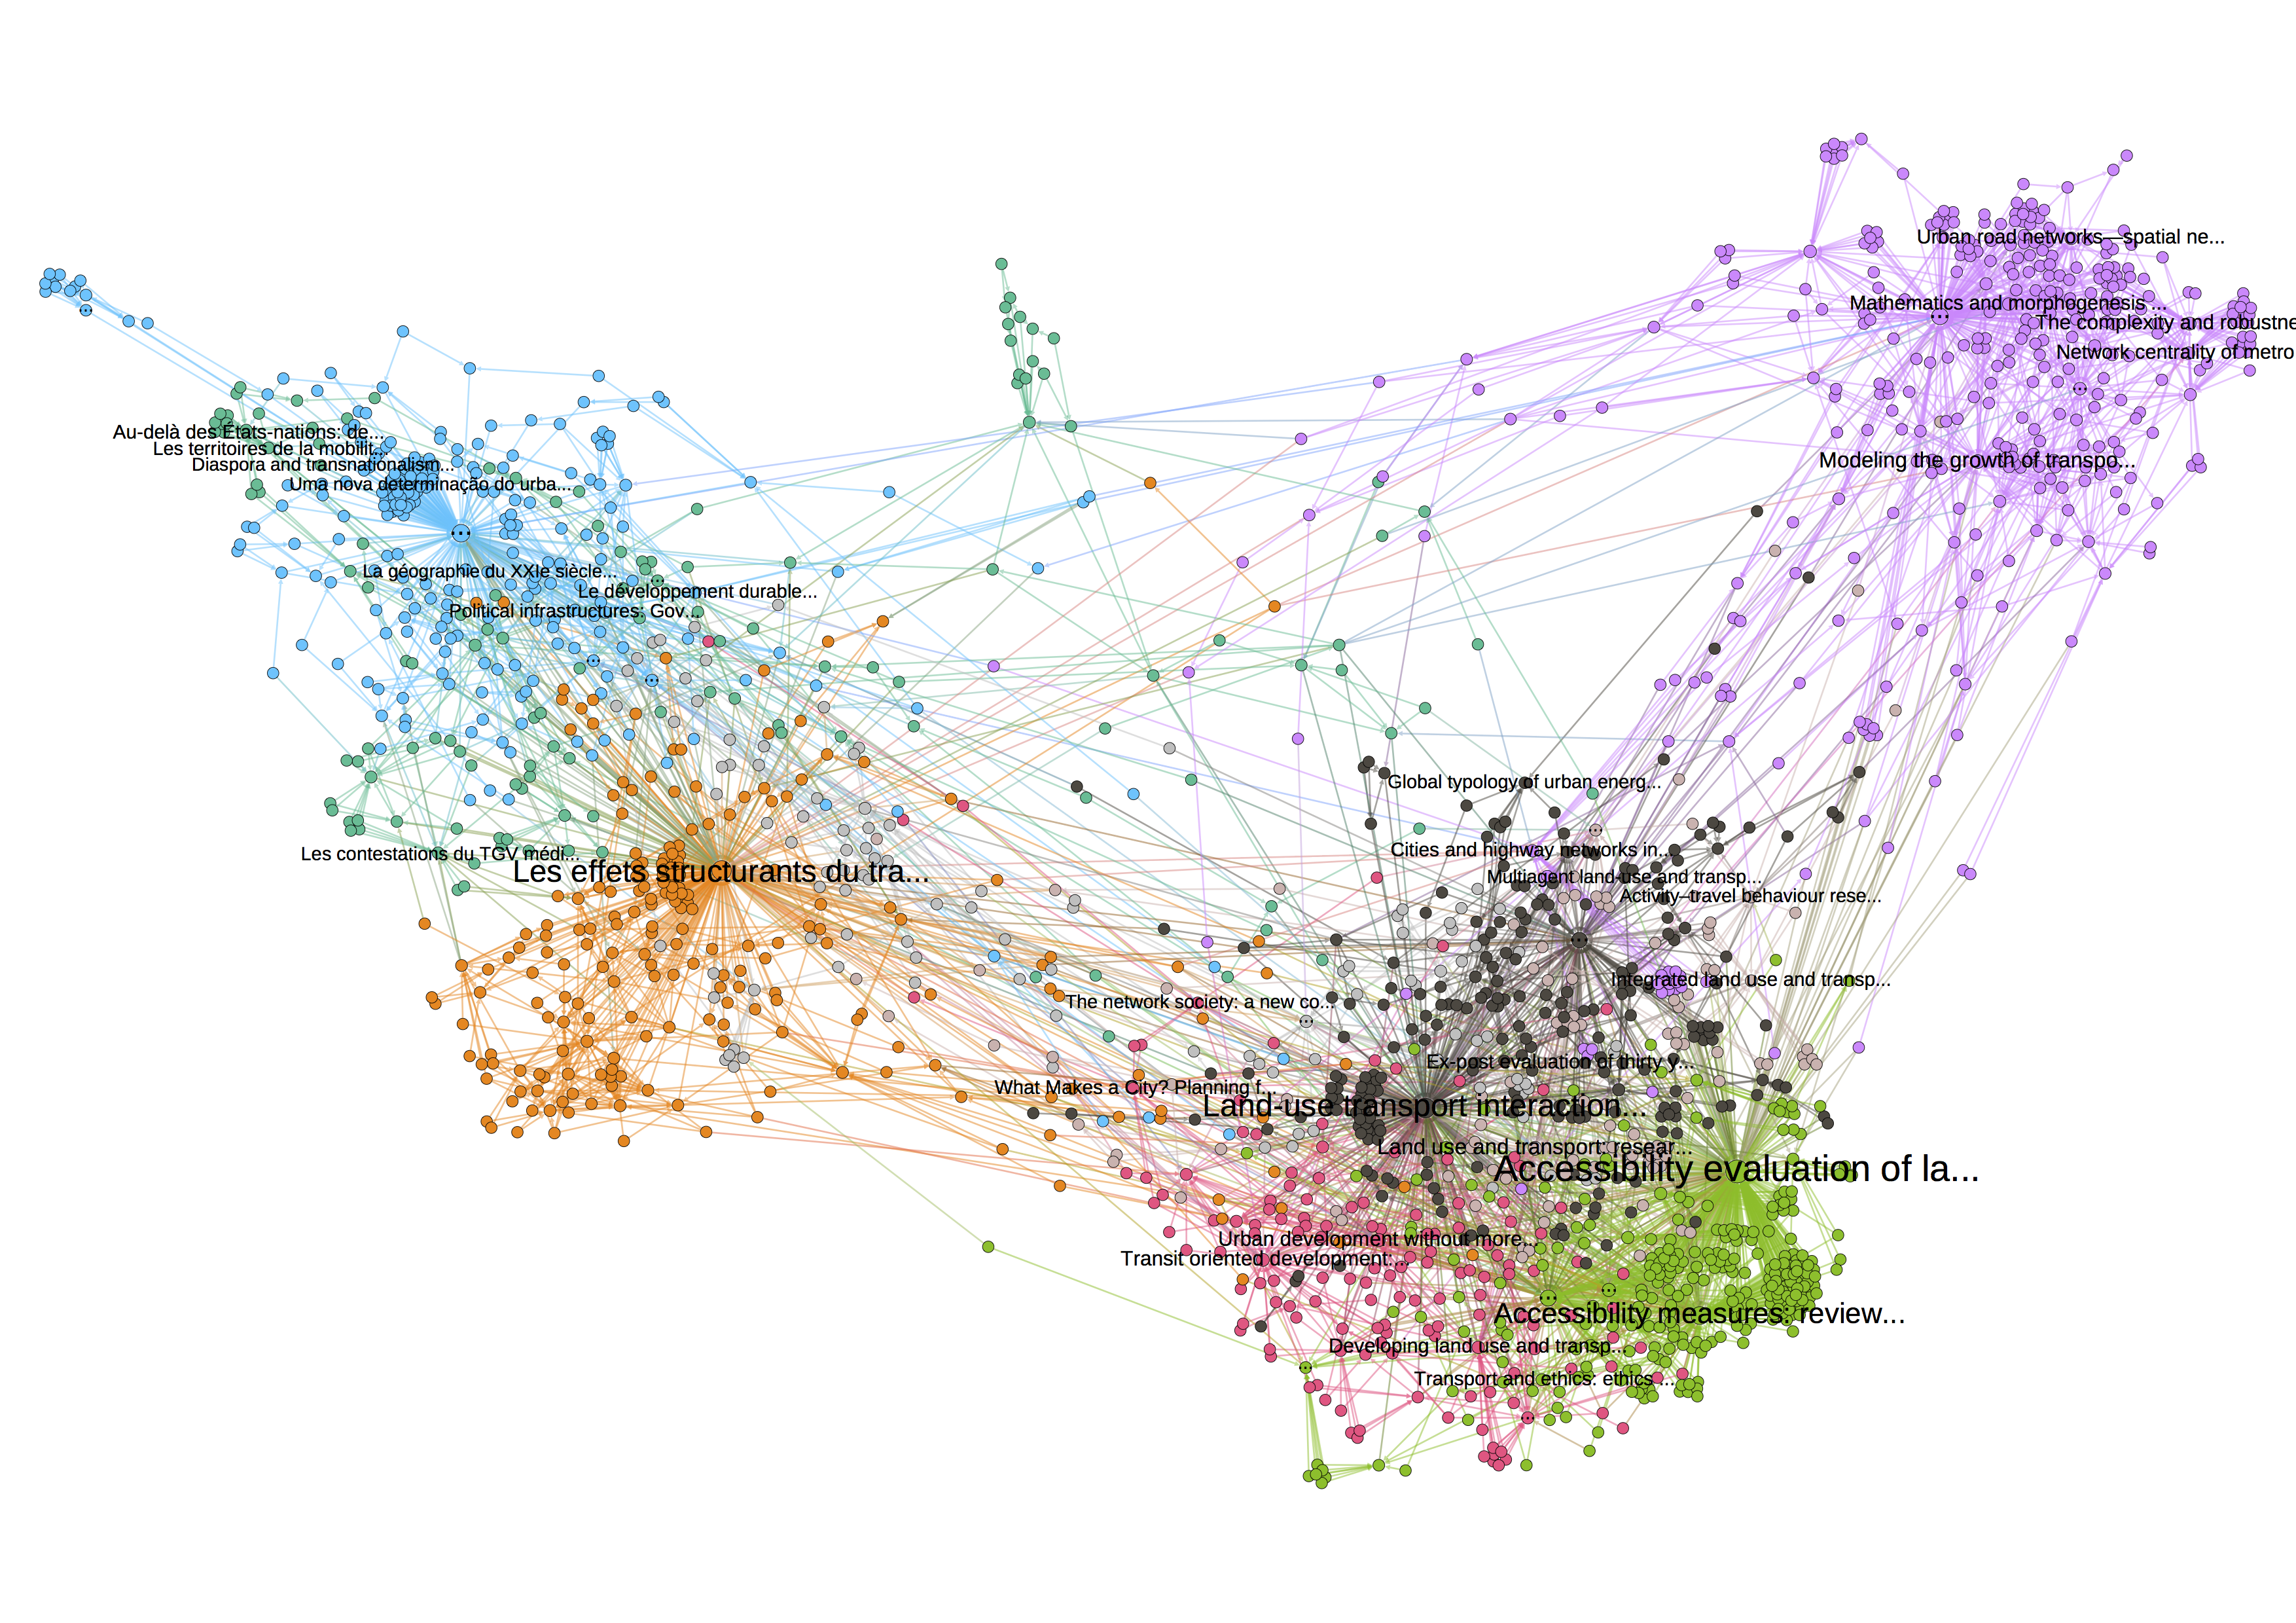
\includegraphics[width=1.25\textwidth]{figures/biblio_rawcore}
\caption{\textbf{Réseau de citations.} A partir d'un ensemble de références, on peut remonter par citation inverse, c'est à dire en récupérant les références citant celles-ci, puis celles les citant, etc. jusqu'à un niveau fixé. Nous montrons ici un réseau à la profondeur 2, construit à partir de domaines scientifiques a priori très disjoints, mais s'intéressant toujours à une approche quantitative des relations entre réseaux et territoires. Les références initiales sont : \cite{offner1996reseaux}, \cite{bretagnolle:tel-00459720}, \cite{offner1993effets} (géographie) ; \cite{wegener2004land} (LUTI) ; \cite{levinson2007co}, \cite{xie2009modeling} (économie) ; \cite{barthelemy2009co} (physique). Le graphe a un degré moyen de 4.76 et une densité de 0.0013. Il est important de noter la connexité. Nous procédons également à une détection de communautés (algorithme de Louvain), qui trouve des sous-ensembles très structurés dans le graphe (modularité de 0.649).}
\label{fig:citnw}
\end{figure}
%%%%%%%%%%%%%%%





%%%%%%%%%%%%%%%%%%
\subsection{Echelle microscopique : des relations chaotiques ?}

Une première entrée consiste à s'intéresser aux processus à une courte échelle temporelle et à une échelle spatiale locale, c'est à dire à des processus typiques des agents fondamentaux desquels émergent les interactions entre transport et territoires. Les utilisateurs d'un réseau routier en sont un exemple typique, puisque la \emph{mobilité} peut être comprise comme une composante fondamentale de l'accessibilité qui s'étudie à une autre échelle. \cite{raimbault2016investigating} étudie les motifs de congestion sur le réseau autoroutier l'Ile-de-France, à granularité temporelle fine (1min), et cherche plus particulièrement à comprendre si les hypothèses d'équilibre et de stationnarité utilisées par la plupart des modèles de trafic sont vérifiées. Certains résultats sont présentés en document~\ref{fig:traffic}.

\medskip

\question{Emettez des hypothèses quand à la modification des plus courts chemins dans le temps ; quelle peut être en général l'amplitude des impacts topologiques d'une disruption d'un lien dans un graphe ; de la même manière les indicateurs que vous connaissez peuvent-ils être très sensibles à une telle disruption ?}

\medskip

\question{Commentez l'évolution temporelle de la variation relative de la centralité d'intermédiarité. Proposez une interprétation concrète de ses valeurs.}

\medskip

\question{Commentez l'évolution temporelle de l'autocorrelation spatiale de la congestion ; en particulier, quelles sont les implications d'une décorrelation sur le caractère chaotique des trajectoires du système ?}



%%%%%%%%%%%%%%%
\begin{figure}
\centering
\includegraphics[width=0.9\textwidth]{figures/traffic_example}\\
\includegraphics[width=0.51\textwidth]{figures/traffic_betweeness}
\includegraphics[width=0.47\textwidth]{figures/traffic_moran}
\caption{\textbf{Analyse spatio-temporelle des motifs de congestion.} \textbf{(Haut)} Exemple de modification d'un plus court chemin en temps de trajet (tiretés bleus), à 10min d'intervalle. La couleur des liens donne le niveau de congestion. \textbf{(Bas Gauche)} Evolution temporelle sur deux semaines de la variabilité de la centralité d'intermédiarité maximale. La centralité d'intermédiarité est définie pour le lien $i$ par $b_i = \frac{1}{N(N-1)}\cdot \sum_{o\neq d \in V}\mathbbm{1}_{i\in p(o\rightarrow d)}$. L'indicateur représenté est alors $\Delta b(t) = \frac{\left|\max_i (b_i(t + \Delta t)) - \max_i (b_i(t))\right|}{\max_i (b_i(t))}$. \textbf{(Bas droite)} Variation temporelle (même fenêtre temporelle) de l'autocorrelation spatiale de la variable de congestion, définie par $c_i = 1 - \frac{t_i}{t_i^{(max)}}$. L'autocorrelation spatiale, estimée ici par Index de Moran, exprime la cohérence spatiale d'une distribution : une valeur tendant vers -1 correspond à une configuration où chaque point s'oppose à ses voisins, une valeur de 0 signifie une configuration aléatoire, et une valeur tendant vers 1 correspond à une configuration homogène. Des phénomènes d'agrégation par voisinage donneront un Moran significativement positif. La courbe violette donne la congestion moyenne, afin de comparer aux moments des heures de pointe.}
\label{fig:traffic}
\end{figure}
%%%%%%%%%%%%%%%






%%%%%%%%%%%%%%%%%%
\subsection{Echelle mesoscopique : Correlations morphologiques et regimes territoriaux ?}

On s'intéresse ici à l'échelle mesoscopique, c'est à dire à celle d'un système métropolitain, intermédiaire entre intra-urbain et système de villes à grande étendue spatiale (même si les transitions entre échelles ne sont jamais évidentes, et que l'échelle peut dépendre du contexte, nécessitant des opérations de \emph{rescaling} pour comparer les systèmes de villes Français et Chinois par exemple ; voir la littérature sur les lois d'échelles urbaines (\emph{urban scaling laws}) pour une entrée sur ces notions que nous n'abordons pas ici). L'hypothèse fondamentale utilisée dans cette section est que la \emph{morphologie}, au sens de \emph{forme urbaine} et \emph{structure du réseau}, joue un rôle fondamental dans les relations à cette échelle. 


\subsubsection{Correlations morphologiques}

% Q : figures here ?

Nous étudions d'abord des données empiriques relativement simples mais contenant un signal riche : la densité de population (raster de résolution 100m) et le réseaux de routes (importé d'OpenStreetMap, simplifié à une résolution équivalente). Cette étude a été présentée dans \cite{raimbault2016cautious}. Le principe est de relier des indicateurs locaux de forme urbaine et de structure de réseau, calculés sur des fenêtres de côté 50km, correspondant à l'échelle à laquelle on s'intéresse. Des tailles voisines (de 25 à 100km) n'influencent pas les résultats de manière significative. Les résultats sont obtenus pour toute l'Europe, mais soulèvent des questions épineuses de comparabilité de qualité des données que nous ne préférons pas aborder ici, étudiant la France uniquement. De même, des indicateurs couplés comme l'accessibilité sont laissés de côté ici pour rester simple. Les documents~\ref{fig:indics-morph} et \ref{fig:indics-nw} montrent les cartes pour certains indicateurs. Le document~\ref{fig:corrs} présente les résultats d'analyses liant les indicateurs de forme urbaine à ceux de réseau, une classification multidimensionelle non-supervisée, et le calcul des corrélations spatiales sur des fenêtres locales.

\medskip

\question{Commentez les distributions des indicateurs de forme urbaine. Quelles structures géographiques semblent intuitives ? Voit-on se dégager de grandes tendances ? Peut-on tirer des conclusions auxquelles on ne s'attendait pas a priori ? Proposez des interprétations.}

\medskip

\question{Faites de même pour les indicateurs de réseau. Voit-on ``à l'oeil nu'' des structures de corrélation se dégager ?}

\medskip

\question{Commentez la distribution spatiale de la classification des profils morphologiques (doc. \ref{fig:corrs}).}

\medskip

\question{Commentez la carte des corrélations. Qu'est ce que différents régimes de correlation impliquent pour la structure des processus urbains à une plus grande échelle (discutez notamment la non-stationnarité) ? [Difficile] L'étude menée ici est entièrement statique ; peut-on imaginer lier correlations spatiales et correlation temporelles sous certaines hypothèses ?}


\bigskip



%%%%%%%%%%%%%%%
\begin{figure}%[h]
\centering
\includegraphics[width=\textwidth]{figures/morpho_indics_morpho_discrquantiles}
\caption{\textbf{Indicateurs de Forme Urbaine.} Les indicateurs sont calculés sur des fenêtres carrées de 50km de côté (sensibilité à la forme du noyau et à sa taille négligeable), placées tous les 10km pour ne pas perdre d'information. L'index de Moran (défini précédemment) donne l'autocorrélation spatiale ; \texttt{distance} est la distance moyenne pondérée par la population ; l'entropie de la distribution donne une mesure de la proximité de la distribution (non spatiale) à une distribution uniforme ; enfin \texttt{slope} donne la pente de la loi rang-taille et traduit le niveau de hiérarchie du système (plus la valeur est négative plus le système est hiérarchisé). La dimension effective est plus faible que le nombre total d'indicateurs, puisque deux composantes principales donnent une variance cumulée de 71\% sur une dimension initiale de 5.}
\label{fig:indics-morph}
\end{figure}
%%%%%%%%%%%%%%%


%%%%%%%%%%%%%%%
\begin{figure}%[h]
\centering
\includegraphics[width=\textwidth]{figures/morpho_indics_network_selected_2_discrquantiles}
\caption{\textbf{Indicateurs de structure de réseau.} Les indicateurs de réseau sont calculés dans des conditions équivalentes à ceux de forme urbaine pour des raisons de comparabilité. \texttt{meanbetweenness} correspond à la moyenne de la centralité d'intermédiarité normalisée, autrement dit plus elle est basse plus le réseau est redondant en chemins alternatifs ; \texttt{alphaCloseness} est le niveau de hiérarchie de la centralité de proximité : plus elle est négative, plus le réseau comporte des points difficiles d'accès ; \texttt{clustCoef} est la moyenne du coefficient de clustering local, qui donne la probabilité que les voisins d'un sommets soient connectés et révèle des structures localement fortement connectées ; enfin \texttt{vcount} est le nombre de sommets du graphe. Ici la dimension effective est plus grande, puisque sur 10 indicateurs les deux premières composantes expliquent 50\% de la variance.}
\label{fig:indics-nw}
\end{figure}
%%%%%%%%%%%%%%%


%%%%%%%%%%%%%%%
\begin{figure}%[h]
%\centering
\hspace{-1cm}
\includegraphics[width=0.55\textwidth]{figures/morpho_cluster_map_k5_full}
\includegraphics[width=0.55\textwidth]{figures/morpho_corr_PCA_rhoasize12}
\caption{\textbf{Analyse couplée entre forme urbaine et structure de réseau.} \textbf{(Gauche)} Typologie morphologique, obtenue par classification non-supervisée en utilisant l'algorithme des \texttt{k-means}. Dans l'espace de l'ensemble des indicateurs, les points proches sont agrégés par iterations pour finalement former un nombre fixé de classes, donnant ainsi des profils typiques. Le choix du nombre de classes peut être délicat, et est effectué ici sur un critère de transition de phase dans le gain d'information lorsqu'une classe supplémentaire est ajoutée : une transition est observée à $k=5$. Les classes de chacune des zones sont cartographiées ici. \textbf{(Droite)} La matrice des correlations locales est calculée pour $n=20$ indicateurs sur une zone rassemblant un certain nombre de zones élémentaires contingentes (228 dans notre cas), donnant une matrice $\rho_{ij}\in \mathcal{M}_n(\left[-1,1\right])$ dont les éléments représentent une ``similarité'' entre indicateurs. Comme cette matrice a $n^2$ éléments ($20\times 20 = 400$ dans notre cas), nous réduisons la dimension par une analyse en composantes principales (28 composantes pour 80\% de la variance), et représentons ici la valeur le long de la première composante (16\% de variance).}
\label{fig:corrs}
\end{figure}
%%%%%%%%%%%%%%%



%%%%%%%%%%%%%%%
\subsubsection{Identifier des régimes de causalité}

Une manière indirecte d'obtenir de l'information sur des interactions similaires mais d'un point de vue dynamique, et de manière stylisée, est d'étudier le comportement d'un modèle de simulation de croissance urbaine contenant certains mécanismes fondamentaux. Le lien entre le poids donnés à certains processus dans le modèle et les régimes de sortie devrait alors pouvoir informer sur le rôle respectif de chaque processus. Le modèle que nous utilisons est un modèle de morphogenèse hybride, décrit et exploré par~\cite{raimbault2014hybrid}. Il correspond typiquement à l'échelle qui nous intéresse. Partant d'un centre urbain initial, de nouveaux arrivants s'établissent prenant en compte certains critères pondérés, dont la densité locale (qui ne doit pas être trop haute), la distance au réseau et la distance au centre (qui doivent être faibles). Des poids $(w_{d},w_{c},w_{r})$ permettent de pondérer l'importance de chaque critère et générer ainsi des formes de villes très différentes, comme illustré au document~\ref{fig:exrdb} : ville compacte, périurbain, ville éclatée, etc. De par les rétroactions entre agents passant par les cellules et le réseau, le résultat final émerge de manière complexe et la valeur finale des indicateurs locaux pour les différents critères ne peuvent pas être prédits à priori, il est donc nécessaire de simuler le modèle pour l'ensemble des paramètres possibles (en le répétant à chaque fois et en prenant la moyenne, celui-ci étant aléatoire). Les \emph{causalités} (au sens de Granger, c'est à dire corrélations retardées) ne sont pas non plus connues a priori et leur valeur devrait nous informer sur les relations entre le réseau et la ville : par exemple une augmentation de la densité cause-t-elle plus tard une croissance du réseau, ou réciproquement. Nous étudions les liens entre densité (\texttt{dens}), distance au centre (\texttt{ctr}) et distance au réseau (\texttt{rd}). Le document~\ref{fig:exrdb} présente les profils moyens sur l'ensemble des patches des correlations retardées pour chaque couple de variables, en fonction du retard $\tau$ variant de $-10$ à $10$. La correlation retardée entre les accroissements des variables $X$ et $Y$ est définie comme $\hat{\rho}\left[\Delta X(t),\Delta Y(t-\tau)\right]$ où $\hat{\rho}$ est un estimateur de Pearson standard (corrélation ``habituelle'') appliqué aux séries temporelles. Une valeur maximale de la correlation retardée de X sur Y à $\tau = 1$ par exemple signifie que $Y$ ``cause'' $X$ avec un décalage temporel d'une unité de temps. En procédant ensuite pour une grille fine dans l'espace des paramètres (pas 0.1), on extrait alors les caractéristiques des courbes $\hat{\rho}(\tau)$ (position et valeurs des maxima et minima), et procède à une classification sur ces caractéristiques. On extrait ainsi des \emph{régimes de causalité}, et le lien de ceux-ci avec la valeur des paramètres de poids des processus nous informe sur le lien entre processus microscopique et interactions émergentes entre réseau et territoire à l'échelle mesoscopique.

\medskip

\question{Commentez les exemples de formes urbaines obtenues par le modèle de simulation (document~\ref{fig:exrdb} ; quelle est la forme du réseau dans chacun des cas, et que pouvez-vous en déduire sur les règles de croissance de réseau ? Cette simplification serait-elle acceptable si on voulait calibrer le modèle de manière couplée sur des données réelles de réseau et de forme urbaine ?}

\medskip

\question{Décrivez les courbes de corrélation retardée en document~\ref{fig:exrdb}. En particulier, voit-on émerger des situations typiques, et pour lesquelles les valeurs correspondantes des paramètres font sens intuitivement ?}

\medskip

\question{Discutez le diagramme de phase des régimes de causalité identifiés par classification non supervisée (document~\ref{fig:clustering}) ; commentez les régimes typiques par les trajectoires de leur centre.}

\bigskip

%%%%%%%%%%%%%%%
\begin{figure}%[h]
\centering
\includegraphics[width=0.29\textwidth]{figures/caus_ex_60_wdens0_wroad1_wcenter1_seed272727}
\includegraphics[width=0.29\textwidth]{figures/caus_ex_60_wdens1_wroad1_wcenter0_seed272727}
\includegraphics[width=0.29\textwidth]{figures/caus_ex_60_wdens1_wroad1_wcenter1_seed272727}\\\vspace{0.2cm}
\includegraphics[width=\textwidth]{figures/caus_laggedcorrs_facetextreme}
\caption{\textbf{Correlations dans le modèle RDB} \textbf{(Première ligne)} Exemples de configurations finales après 60 pas de temps, obtenues avec $(w_{d},w_{c},w_{r})$ valant respectivement $(0,1,1)$,$(1,0,1)$, et $(1,1,1)$. \textbf{(Deuxième ligne)} Corrélations retardées, pour chaque combinaison des paramètres (valeurs de $(w_{d},w_{c},w_{r})$ en en-tête de chaque graphe), en fonction du retard $\tau$. Les différentes couleurs correspondent à chaque couple de variables.}
\label{fig:exrdb}
\end{figure}
%%%%%%%%%%%%%%%




%%%%%%%%%%%%%%%
\begin{figure}%[h]
%\centering
\hspace{-1cm}
\includegraphics[width=0.36\textwidth]{figures/caus_ccoef-knum_valuesFALSE_theta05-3.pdf}
\includegraphics[width=0.36\textwidth]{figures/caus_dccoef-knum_valuesFALSEtheta05-3.pdf}
\includegraphics[width=0.28\textwidth]{figures/caus_clusters-PCA-features_valuesFALSEtheta2_k6}\\\hspace{-1cm}
\includegraphics[width=0.5\textwidth]{figures/caus_clusters-paramfacet_valuesFALSEtheta2_k6}
\includegraphics[width=0.58\textwidth]{figures/caus_clusters-centertrajs-facetclust_valuesFALSEtheta2_k6}
\caption{\textbf{Identification de régimes d'interactions} \textbf{(Haut Gauche)} Variance inter-cluster comme fonction du nombre de clusters, pour différentes valeurs du paramètre $\theta$ de filtration des \emph{features} (caractéristiques des courbes). \textbf{(Haut Milieu)} Dérivée de la variance inter-cluster. Avec le graphe précédent, ces deux courbes permettent de fixer le nombre de classe, à la transition observée à $k=6$. \textbf{(Haut Droite)} Features dans un plan principal, permettant de visualiser les classes formées. \textbf{(Bas Gauche)} Diagramme de phase des régimes dans l'espace $(w_{d},w_{c},w_{r})$ exploré entièrement par une grille de pas 0.1. Chaque diagramme donne la classe comme fonction de $(w_d,w_c)$ à $w_r$ fixé (donnée en en-tête). \textbf{(Bas Droite)} Trajectoires correspondantes des centres des classes, permettant d'interpréter à quel type de régime correspond chaque classe.}
\label{fig:clustering}
\end{figure}
%%%%%%%%%%%%%%%






%%%%%%%%%%%%%%%%%%
\subsection{Echelle macroscopique : Effets structurants ?}

Enfin, une dernière entrée est donnée par un modèle de croissance urbaine pour un système de villes, à l'échelle macroscopique, considérant les villes comme des agents en interaction, influençant chacun leur processus de croissance de population. Les résultats présentés ici sont donnés de manière préliminaire par \cite{raimbault2016models}. Le modèle est encore très simple, ne prenant en compte que la variable de la population des villes. On s'intéresse au système de ville français entre 1831 et 1999 (base de données Pumain-INED). Le modèle est une variante du Favaro-Pumain~\cite{favaro2011gibrat} qui étend le modèle de Gibrat en ajoutant la diffusion de l'innovation entre les villes comme moteur de la croissance. Dans notre cas, la composante particulière s'ajoutant aux termes de croissance endogène et d'interaction gravitaire est un terme lié à l'effet du réseau. Plus particulièrement, le modèle s'écrit, si $\vec{\mu}(t)$ est le vecteur des populations à l'année $t$, sous la forme

\begin{equation}
\vec{\mu}(t+1) = r_0\cdot \mathbf{Id}\cdot \vec{\mu}(t) + \mathbf{G}\left(\vec{\mu}(t)\right)\cdot \mathbf{1} + \mathbf{N}\left(\vec{\mu}(t)\right)
\end{equation}


avec $G_{ij} = w_G\cdot \frac{V_{ij}}{<V_{ij}>}$ de telle sorte que le potentiel d'interaction suive une interaction de type gravitaire donnée par

\begin{equation}
G_{ij} = \left(\frac{\mu_i\mu_j}{\sum{\mu_k}^2}\right)^{\gamma_G}\cdot \exp{(-d_{ij}/d_G)}
\end{equation}

et le terme traduisant l'effet du réseau est donné par


\begin{equation}
N_{i} = w_N \cdot \sum_{kl} \left(\frac{\mu_k\mu_l}{\sum\mu}\right)^{\gamma_N}\exp{(-d_{kl,i}/d_N)}
\end{equation}

où $d_{kl,i}$ est la distance de $i$ au plus court chemin dans le réseau entre $k$ et $l$. Pour isoler les effets structurants des flux de particularités liées à la croissance du réseau qui est fortement dépendante au chemin, nous choisissons d'utiliser des plus courts chemins géographiques, calculés à partir du modèle numérique de terrain à 1km avec une impédance lié à la dénivellation donnée par $Z=\left(1+\alpha/\alpha_0\right)^{n_0}$ avec $\alpha_0\simeq 3$ et $n_0 = 3$. L'interprétation de chaque composante est la suivante : la première est un taux de croissance endogène à chaque ville, dépendant uniquement de la population. Le deuxième traduit une interaction spatiale qui s'atténue avec la distance, pouvant être vue comme des flux de migrations. La composante de réseau suppose que les \emph{flux} ont un impact sur les territoires qu'ils traversent : si $i$ est situé non loin de la route reliant $k$ à $l$, alors le passage de cette route aura une influence sur sa croissance. On peut penser à Dijon qui a tiré parti de sa position centrale au sein des réseaux classiques, mais que les nouveaux réseau (TGV et autoroute) ne placent pas aussi bien. Le modèle est calibré sur une fenêtre temporelle glissante de 50ans, avec pour objectifs de calibration le logarithme de l'erreur au carré moyenne (privilégie la justesse sur les grandes villes) et l'erreur au carré moyenne sur les logarithmes (privilégie la justesse relative sur l'ensemble des villes), entre les populations simulées et les populations réelles. Cette hypothèse de stationnarité temporelle locale est confortée par l'analyse empirique des données (voir document~\ref{fig:macro}). Les résultats de calibration du modèle, notamment au regard de la composante réseau, devraient informer sur l'influence du réseau (de manière abstraite puisque sa forme réelle n'est pas prise en compte) dans les processus de croissance des villes. Par rapport à l'approche précédente, les notions morphologiques ne sont plus prépondérantes à cette échelle.

\medskip

\question{Discutez les courbes empiriques des taux de croissances à différentes dates en fonction de la distance. En particulier, leur évolution peut-elle être mise en parallèle à de grandes étapes d'évolution des réseaux de transports ?}

\medskip

\question{Discutez la calibration du modèle gravitaire seul (sans composante de réseau). L'influence de la distance semble-t-elle cohérente avec les observations empiriques ?}

\medskip

\question{Discutez les implications de la forme des courbes de calibration avec la composante réseau, en particulier sur le pouvoir explicatif supplémentaire apporté par la prise en compte des flux. Comment pourrait-on alors tirer parti de la valeur des paramètres calibrés, par exemple de la distance caractéristique d'influence des flux ? ([indice] : par exemple, quel lien avec l'effet tunnel ?) Ce travail est encore en cours car des difficultés se posent lors de la calibration du modèle complet : en effet, peut-on être toujours sûr que l'ajout de mécanismes n'améliore pas le pouvoir explicatif du modèle juste par l'ajout de degrés de liberté supplémentaires (phénomène d'overfitting) ?}


%%%%%%%%%%%%%%%
\begin{figure}%[h]
\centering
\includegraphics[width=0.48\textwidth]{figures/macro_empirical_tsCorrelations}
\includegraphics[width=0.48\textwidth]{figures/macro_gravity}\\
\includegraphics[width=0.48\textwidth]{figures/macro_argmins_gravityDecay}
\includegraphics[width=0.48\textwidth]{figures/macro_mselog-feedbackDecay_ZOOM_fixedgravity}
\caption{\textbf{Modèle macroscopique d'interactions spatiales.} \textbf{(Haut Gauche)} Correlations entre séries temporelles des taux de croissance normalisés de population des villes, calculées sur des fenêtres glissantes de 50ans (la légende donne la fin de la période). La valeur moyenne de la correlation sur l'ensemble des couples est représentée en fonction de la distance entre les villes, le graphe montrant ainsi les distances typiques d'interaction et leur évolution dans le temps. \textbf{(Haut Droite)} Calibration du modèle sans réseau (deux premières composantes seulement) : les points représentés sont les meilleures solution au sens de Pareto pour les deux objectifs de calibration contradictoires (\emph{Front de Pareto}), pour chacune des sous-périodes temporelles. La couleur donne la valeur du paramètre de distance d'interaction correspondante. Les périodes 1891-1911 et 1946-1968 saturent ce paramètre et sont à interpréter avec précaution. \textbf{(Bas Droite)} Valeur moyenne et déviation standard de ce paramètre en fonction du temps, pour des optimisations uniobjectif (\texttt{logmse} et \texttt{mselog}) et sur l'ensemble du front de Pareto (\texttt{pareto}). Ce graphe peut être interprété comme l'évolution temporelle de la distance typique d'interaction entre villes. \textbf{(Bas Droite)} Etape préliminaire de calibration du modèle complet : à paramètres de Gibrat et de gravité fixés, valeur de l'erreur \texttt{mselog} en fonction de la distance typique d'influence des flux $d_N$ (\texttt{feedbackDecay}), pour différentes valeurs du rapport des poids $w_N/w_G$. L'existence de ce minimum stable pour l'ensemble des poids suggère l'existence \emph{d'effets de réseaux}.}
\label{fig:macro}
\end{figure}
%%%%%%%%%%%%%%%


%%%%%%%%%%%%%%%%%%
\subsection{Ouverture épistémologique}

La question précédente est une question ouverte pour les modèles de simulation complexe (résolue par exemple pour les modèles statistiques). Pour y répondre, on a élaboré et testé une nouvelle méthodologie (critère d'Information d'Akaike empirique). De même, les analyses bibliométriques ont nécessité la mise au points de nouvelles méthodes et de nouveau outils, comme pour les analyses mesoscopiques morphologiques. L'étude du traffic a impliqué une collecte de donnée par moissonnage et la création d'une base de données non existante. Les modèles et les constructions théoriques interagissent avec chacun de ces éléments et s'en enrichissent, mais aussi leur apportent de nouvelle questions ou éléments de réponse. Les \emph{domaines de connaissance} au sujet d'objet complexes seraient en \emph{co-évolution}, dans le cadre d'une compréhension perspectiviste des sciences~\cite{giere2010scientific}. En effet, cette approche cognitive de la production de connaissance met au centre de celle-ci les agents qui la produisent (les scientifiques), qui ont alors chacun une perspective, qui contient un but, un objet réel étudié, et un medium pour arriver au but (qu'on appelle alors le \emph{modèle}). Cette vision par perspective est une voie différente des dichotomies classiques entre réalisme et constructivisme. Elle est totalement compatible avec notre approche par domaines de connaissance co-évolutifs, considérant tout processus de production de connaissances complexes comme un processus co-évolutif entre domaines et agents. Une ébauche de ce cadre de connaissances a été présentée par~\cite{raimbault:halshs-01505084}. Celui-ci ouvre des perspectives vers des sciences territoriales plus intégrées, au sens des disciplines, des niveaux et de la relation quantitatif-qualitatif, c'est à dire la possibilité d'une \emph{géographie intégrée} qui est en fait pratiquée par la majorité de la Géographie Théorique et Quantitative depuis une trentaine d'années, et dont la construction de la Théorie Evolutive des Villes en est l'illustration parfaite (voir par exemple \cite{pumain1997pour}, \cite{sanders1997simpop} pour les précurseurs, et \cite{pumain2017urban} pour les accomplissements les plus récents).

\medskip

\question{Proposez des exemples de connaissances géographiques dans des domaines variés pouvant illustrer cette lecture de la production de connaissances.}

\medskip

{\centering
$\star$ \hspace{1cm}$\star$\\
\medskip
\hfill$\star$\hfill
}


%%%%%%%%%%%%%%%
\begin{figure}%[h]
\centering
\includegraphics[width=0.8\textwidth]{figures/epistemo_tqg}
\caption{\textbf{Représentation simplifiée des domaines de connaissance en co-évolution.} La qualification des relations binaires cherche à donner une idée de la nature des relations possibles, mais ne correspond généralement pas à ce qui se passe en réalité, puisque certains domaines peuvent agir en catalyseurs pour la relation entre d'autres, et que la co-évolution se passe entre plus de deux domaines.}
\label{fig:clustering}
\end{figure}
%%%%%%%%%%%%%%%





%%%%%%%%%%%%%%%%%%
\bibliographystyle{apalike-fr}
\bibliography{/Users/Juste/Documents/ComplexSystems/CityNetwork/Biblio/BibTeX/CityNetwork,biblio}





\end{document}